\section*{Assignment 4}
% Pin 
% resetting fpga, tou cut the time when fpga was responding wrong PW
% the rest was implemented via python, and tee Fpga worked as Translator

% \emph{Aufgabe: }We had an FPGA configured by the tutors. We should enter it, without any Knowledge what it does.

This time, we only get one pre programmed micro controller with a single UART communication interface. 
To figure out the functionality of the device and how we could possibly attack it, we connect it to the computer and perform a black box analysis.
After powering up, the device expects four input bytes via UART, answers \textit{``Incorrect PIN"} and imposes a 10 second penalty upon the input of the next four bytes. Now the task at hand is clear -- we have to obtain the correct PIN.

We begin by setting the FPGA up in between computer and micro controller, letting it relay the communication passively, like in assignment 3.
To get past the timing penalties, we add a receiver to the design, locate the micro controller's \texttt{rst} pin and connect it to the FPGA, so that it can be triggered whenever the computer transmits a special command byte, thus making brute force approaches feasible.

From this point on, we pursue two different paths to solve the task.

\subsubsection*{An easy solution}
Following the first direction, the FPGA does not need any further programming, see figure \ref{fig:as4-schematic-1} (p.~\pageref{fig:as4-schematic-1}) for a schematic of the final setup. Instead, we just write and execute a script in the high-level language Python on the computer. It takes about 30 seconds to obtain the correct PIN by iterating over all possibilities, 0000--9999, and telling the FPGA to reset the device, if the given PIN is wrong.

\begin{figure}[htb]
    \begin{center}
        \usetikzlibrary{arrows.meta}
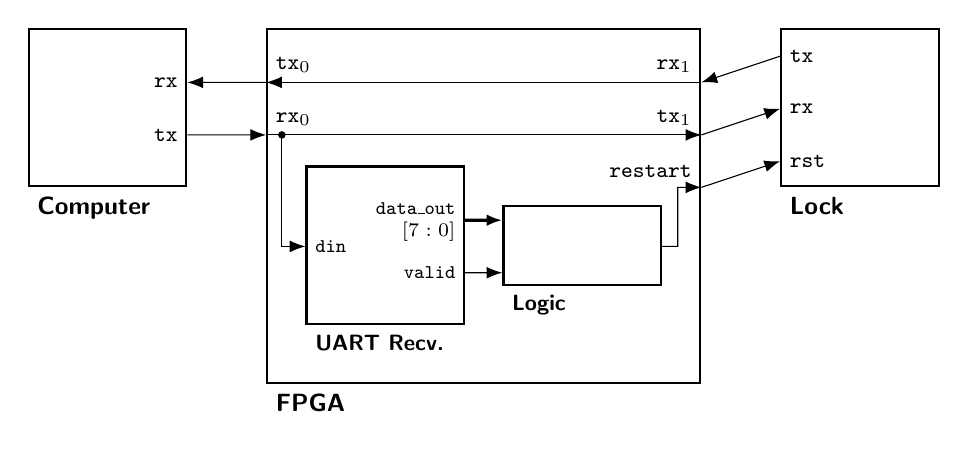
\begin{tikzpicture}
	\tikzstyle{comp} = [
		rectangle, draw=black, thick
	]
	\tikzstyle{component} = [
		comp, minimum width=5.5cm, minimum height=4.5cm
	]
\tikzstyle{component_small} = [
		comp, minimum width=2cm, minimum height=2cm
	]
	\tikzstyle{caption} = [
		below right
	]
	\tikzstyle{conn} = [
		-{Latex[length=2mm]}
	]
	
	% FPGA
	\node (FPGA) [component] at (0,0) {}
		% Caption
		node [caption] at (FPGA.south west) { \small{\textsf{\textbf{FPGA}}} }
		% In/-outputs links
		coordinate [yshift=2.5cm+0.666cm, label={ above right : \footnotesize{$\texttt{rx}_0$} }] (FPGA_rx0) at (FPGA.south west) % unten
		coordinate [yshift=2.5cm+1.333cm, label={ above right : \footnotesize{$\texttt{tx}_0$} }] (FPGA_tx0) at (FPGA.south west) % oben
		% In/outputs  rechts
		coordinate [yshift=2.5cm,                    label={ above left : \footnotesize{$\texttt{restart}$} }] (FPGA_restart) at (FPGA.south east) % unten
		coordinate [yshift=2.5cm+0.666cm, label={ above left : \footnotesize{$\texttt{tx}_1$} }]      (FPGA_tx1)        at (FPGA.south east) % mitte
		coordinate [yshift=2.5cm+1.333cm, label={ above left : \footnotesize{$\texttt{rx}_1$} }]      (FPGA_rx1)        at (FPGA.south east)  % oben
	;

	% Receiver
	\node (Receiver) at (FPGA.south west) [component_small, above right, shift={(0.5, 0.75)}] {}
		% Caption
		node [caption] at (Receiver.south west) { \textsf{\footnotesize{\textbf{UART Recv.}}} }
		% Input rechts
		coordinate [yshift=1cm, label={ right : \scriptsize{\texttt{din}} }] (Receiver_din) at (Receiver.south west)
		% Outpus rechts
		coordinate [yshift=0.666cm,                 label={ left : \scriptsize{\texttt{valid}} }]           (Receiver_valid)           at (Receiver.south east) % unten
		coordinate [yshift=1.333cm+0.15cm, label={ left : \scriptsize{\texttt{data\_out}} }] (Receiver_data_out)    at (Receiver.south east) % oben
		coordinate [yshift=1.333cm-0.15cm,  label={ left : \scriptsize{$[7:0]$} }]                     (Receiver_data_out2) at (Receiver.south east) % mitte
	;

	% Logic
	\node (Logic) at (FPGA.south east) [comp, minimum height=1cm, minimum width=2cm, above left, shift={(-0.5, 1.25)}] {}
		node [caption] at (Logic.south west) { \textsf{\footnotesize{\textbf{Logic}}} }
		% Inputs rechts
		coordinate [yshift=0.166cm] (Logic_in0) at (Logic.south west) % unten
		coordinate [yshift=0.833cm] (Logic_in1) at (Logic.south west) % oben
		% Output link
		coordinate [yshift=0.5cm] (Logic_out) at (Logic.south east)
	;

	% Computer
	\node (Computer) [component_small, below left, xshift=-1cm] at (FPGA.north west) {}
		% Caption
		node [caption] at (Computer.south west) { \small{\textsf{\textbf{Computer}}} }
		% In/outputs rechts
		coordinate [yshift=0.666cm, label={ left:\footnotesize{\texttt{tx}} }] (Computer_tx) at (Computer.south east) % unten
		coordinate [yshift=1.333cm, label={ left:\footnotesize{\texttt{rx}} }] (Computer_rx) at (Computer.south east) % oben
	;

	% Lock
	\node (Lock) [component_small, below right, xshift=1cm] at (FPGA.north east) {}
		% Caption
		node [caption] at (Lock.south west) { \small{\textsf{\textbf{Lock}}} }
		% In/outputs rechts
		coordinate [yshift=0.333cm, label={ right:\footnotesize{\texttt{rst}} }] (Lock_rst) at (Lock.south west) % unten
		coordinate [yshift=0.999cm, label={ right:\footnotesize{\texttt{rx}} }]   (Lock_rx)   at (Lock.south west) % mitte
		coordinate [yshift=1.666cm, label={ right:\footnotesize{\texttt{tx}} }]   (Lock_tx)   at (Lock.south west) % oben
	;

	% Computer -> FPGA
	\draw[conn] (Computer_tx) -- (FPGA_rx0);
	\draw[conn] (FPGA_tx1) -- (Lock_rx);
	\draw[conn] (FPGA_restart) -- (Lock_rst);
	
	% FPGA -> Computer
	\draw[conn]  (Lock_tx) -- (FPGA_rx1) ;
	\draw[conn]  (FPGA_tx0) -- (Computer_rx);
	
	% FPGA internal
	\draw[conn] (FPGA_rx0) -- (FPGA_tx1);
	\draw[conn]  (FPGA_rx1) -- (FPGA_tx0);
	\draw[fill=black] (FPGA_rx0) +(0.2,0) circle (0.4mm);
	\draw[conn] (FPGA_rx0) +(0.2,0) |- (Receiver_din);
	\draw[conn] (Receiver_valid) -- (Logic_in0);
	\draw[conn, very thick] (Receiver_data_out) +(0, -0.15) -- (Logic_in1);
	\coordinate [xshift=0.2cm] (h1) at (Logic_out);
	\coordinate [yshift=0.75cm] (h2) at (h1);
	\draw[conn] (Logic_out) -- (h1) -- (h2) -- (FPGA_restart);

\end{tikzpicture}
        \caption{In this setup, all possible PINs are computed on the computer and transmitted to the device. The FPGA just relays the communication and understands the computer's output bitstream to reset the mircrocontroller upon receiving a special command.}
        \label{fig:as4-schematic-1}
        \vspace{1em}\hrule
    \end{center}
\end{figure}


\subsubsection*{The fast way}
From a hardware engineering perspective, this first method is rather boring. We (probably) did not even use a tiny part of the FPGA's ressources. 
But we can change this and harness its full potential: by moving all workload to the FPGA, effectively reducing the computer to a mere replaceable output device. 

In order to do so, we begin with rewiring the receiver to listen to the micro controller's output.
Next, we program the FPGA to reset the device on its own, whenever it receives the ASCIIbyte $49_{16}$, `I', as in \textit{``Incorrect PIN"}, first. 
To be able to send PINs, we add a transmitter, which output is connected to both, the computer's and the micro controller's, \texttt{rx} lines. 
See figure \ref{fig:as4-schematic-2} (p.~\pageref{fig:as4-schematic-2}) for a schematic of the arrangement at this point.
Now, we only have to port the brute force algorithm, i.~e., generation and transmission of all possible PINs, to run in the logic on the FPGA. We achieve this with the following finite 4-state machine.

\begin{itemize}
    \item[] \begin{labeling}{\textsc{Receive}:}
        \item[\textsc{Start}:] Initialise the PIN to 0000, treating every digit as its own byte in a four byte array;\\go to \textsc{Send}.
        \item[\textsc{Send}:] Transmit the most significant byte of the PIN and rotate it one byte to the left (this is repeated four times to transmit every digit);\\go to \textsc{Inc}.
        \item[\textsc{Inc}:] Increment the most significant byte of the PIN by one, passing possible carryovers to the next bytes;\\go to \textsc{Receive}.
        \item[\textsc{Receive}:] If the device's answer does not start with `I', do nothing, otherwise reset the micro controller and go to \textsc{Send}.
    \end{labeling}
\end{itemize}

Since transmission of the generated PINs reaches both, micro controller and computer, we just have to start a program that can read serial input from a USB port, like \texttt{screen}, before starting the attack and the last four digits of the printed output are the correct PIN. Obtaining it takes only about 3 seconds and thus, compared to the first approach, this one is magnitudes faster.

\begin{figure}[tb]
    \begin{center}
        \usetikzlibrary{arrows.meta}
\usetikzlibrary{calc,intersections,through,backgrounds}
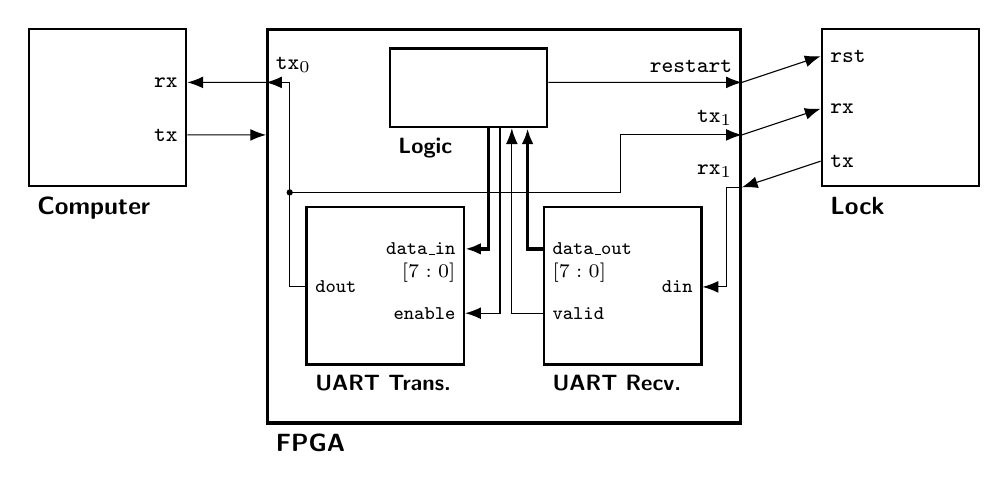
\begin{tikzpicture}
% 	\tikzset{
% 	  every node/.style={scale=1.1}
% 	}	
	\tikzset{comp/.style={
		rectangle, draw=black, thick
	}}	
	\tikzset{component/.style={
		comp, minimum width=6cm, minimum height=5cm, very thick
	}}
	\tikzset{component_small/.style={
		comp, minimum width=2cm, minimum height=2cm, thick
	}}
	\tikzset{caption/.style={
		below right
	}}
	\tikzset{conn/.style={
		-{Latex[length=2mm]}
	}}
	
	% FPGA
	\node (FPGA) [component] at (0,0) {}
		% Caption
		node [caption] at (FPGA.south west) { \small{\textsf{\textbf{FPGA}}} }
		
		% In/-outputs links
		coordinate [yshift=3cm+0.4pt+0.666cm, label={ above right : \footnotesize{} }]                           (FPGA_rx0) at (FPGA.south west) % unten
		coordinate [yshift=3cm+0.4pt+1.333cm, label={ above right : \footnotesize{$\texttt{tx}_0$} }] (FPGA_tx0) at (FPGA.south west) % oben

		% In/outputs  rechts
		coordinate [yshift=3cm+0.4pt,                    label={ above left : \footnotesize{$\texttt{rx}_1$} }]      (FPGA_rx1)       at (FPGA.south east)  % unten
		coordinate [yshift=3cm+0.4pt+0.666cm, label={ above left : \footnotesize{$\texttt{tx}_1$} }]      (FPGA_tx1)       at (FPGA.south east) % mitte
		coordinate [yshift=3cm+0.4pt+1.333cm, label={ above left : \footnotesize{$\texttt{restart}$} }] (FPGA_restart) at (FPGA.south east) % oben
	;

	% Logic
	\node (Logic) at (FPGA.north) [comp, minimum height=1cm, minimum width=2cm, below, shift={(-0.45cm, -0.25cm)}] {}
		node [caption] at (Logic.south west) { \textsf{\footnotesize{\textbf{Logic}}} }
	;

	% Receiver
	\node (Receiver) at (FPGA.south east) [component_small, above left, shift={(-0.5, 0.75)}] {}
		% Caption
		node [caption] at (Receiver.south west) { \textsf{\footnotesize{\textbf{UART Recv.}}} }

		% Input rechts
		coordinate [yshift=1cm, label={ left : \scriptsize{\texttt{din}} }] (Receiver_din) at (Receiver.south east)

		% Outpus links
		coordinate [yshift=0.666cm,                 label={ right : \scriptsize{\texttt{valid}} }]           (Receiver_valid)           at (Receiver.south west) % unten
		coordinate [yshift=1.333cm+0.15cm, label={ right : \scriptsize{\texttt{data\_out}} }] (Receiver_data_out)    at (Receiver.south west) % oben
		coordinate [yshift=1.333cm-0.15cm,  label={ right : \scriptsize{$[7:0]$} }]                     (Receiver_data_out2) at (Receiver.south west) % mitte
	;

	% Transmitter
	\node (Transmitter) at (FPGA.south west) [component_small, above right, shift={(0.5, 0.75)}] {}
		node [caption] at (Transmitter.south west) { \textsf{\footnotesize{\textbf{UART Trans.}}} }

		% Output links
		coordinate [yshift=1cm, label={ right: \scriptsize{\textsf{\texttt{dout}}} }] (Transmitter_dout) at (Transmitter.south west) % unten

		% Inputs links
		coordinate [yshift=0.666cm,                 label={ left : \scriptsize{\texttt{enable}} }]    (Transmitter_enable)   at (Transmitter.south east) % unten
		coordinate [yshift=1.333cm-0.15cm,  label={ left : \scriptsize{$[7:0]$} }]                  (Transmitter_data_in2)at (Transmitter.south east) % mitte
		coordinate [yshift=1.333cm+0.15cm, label={ left : \scriptsize{\texttt{data\_in}} }] (Transmitter_data_in)  at (Transmitter.south east) % oben	
	;

	% Computer
	\node (Computer) [component_small, below left, xshift=-1cm] at (FPGA.north west) {}
		% Caption
		node [caption] at (Computer.south west) { \small{\textsf{\textbf{Computer}}} }

		% In/outputs rechts
		coordinate [yshift=0.666cm, label={ left:\footnotesize{\texttt{tx}} }] (Computer_tx) at (Computer.south east) % unten
		coordinate [yshift=1.333cm, label={ left:\footnotesize{\texttt{rx}} }] (Computer_rx) at (Computer.south east) % oben
	;

	% Lock
	\node (Lock) [component_small, below right, xshift=1cm] at (FPGA.north east) {}
		% Caption
		node [caption] at (Lock.south west) { \small{\textsf{\textbf{Lock}}} }

		% In/outputs rechts
		coordinate [yshift=0.333cm, label={ right:\footnotesize{\texttt{tx}} }]   (Lock_tx)   at (Lock.south west) % unten
		coordinate [yshift=0.999cm, label={ right:\footnotesize{\texttt{rx}} }]   (Lock_rx)   at (Lock.south west) % mitte
		coordinate [yshift=1.666cm, label={ right:\footnotesize{\texttt{rst}} }] (Lock_rst)  at (Lock.south west) % oben
	;

	% Computer <-> FPGA
	\draw[conn]  (FPGA_tx0) -- (Computer_rx);
	\draw[conn] (Computer_tx) -- (FPGA_rx0);

	% FPGA <-> Lock
	\draw[conn] (FPGA_restart) -- (Lock_rst);
	\draw[conn] (FPGA_tx1) -- (Lock_rx);
	\draw[conn] (Lock_tx) -- (FPGA_rx1) ;
	
	% FPGA internal
		\draw[conn] ([yshift=0.583cm] Logic.south east) -- (FPGA_restart);
	
		% Connections to/from Receiver
		\draw[conn] (FPGA_rx1) -- ([xshift=-0.2cm] FPGA_rx1) |- (Receiver_din);
		\draw[conn, very thick] (Receiver_data_out) -| ([xshift=0.75cm] Logic.south); 
		\draw[conn] (Receiver_valid) -| ([xshift=0.55cm] Logic.south);
		
		% Connections to/from Transmitter
		\draw[conn, very thick] ([xshift=0.25cm]Logic.south) |- (Transmitter_data_in);
		\draw[conn] ([xshift=0.4cm] Logic.south) |- (Transmitter_enable);
		\draw[conn, name path=Transmitter_dout--FPGA_tx0] (Transmitter_dout) -- ([xshift=-0.2cm] Transmitter_dout) |- (FPGA_tx0);
		\draw[conn, name path=Transmitter_dout--FPGA_tx1] ([shift={(-0.2cm, 1.2cm)}] Transmitter_dout) -- ([shift={(4cm, 1.2cm)}] Transmitter_dout) |- (FPGA_tx1);

		% Intersection
		\fill[name intersections={of=Transmitter_dout--FPGA_tx0 and Transmitter_dout--FPGA_tx1, total=\t}] (intersection-\t) circle (0.4mm);
\end{tikzpicture}
        \caption{Now the FPGA calculates the 4 digit numbers, sends them to the device and decodes the answer bitstream in order to reset the microcontroller. The computer is passive in this configuration and only needed as an output device, thus we ignore its transmissions.}
        \label{fig:as4-schematic-2}
        \vspace{1em}\hrule
    \end{center}
\end{figure}




%\emph{Bearbeitung und Lösung: }
%Um den Brutforce algorythmus auf dem FPGA zu realisieren, Bauten wir eine State Mashine mit 4 Zuständen, einem UART-Transmitter und einem UART-Reciver.

%\begin{itemize}
    %\item[START] Ist der erste Zustand der STate mashine, in dem die 4 stellen des Pins sowie einem 5. Übertragszahl auf 0 gesetzt. diese 5 Ziffern werden als 8-Bit gehandhabt. Außerdem werden andere Register initialisiert.

    %\item[SEND] In diesem Zustand das erste Byte des 4 Stelligen Pins an den UART-Tranmitter übergeben, welcher es direkt an die FPGA-Pin weiterleitet. nun werden alle stellen des Pins um eine stelle verrückt, wobei die vorher erste stelle auf die Hilfvariable übertragen wird. Nun wird der Vorgang wiederholt und die neue erste Stelle des Pins via Transmitter übermittelt. Dieser vorgang findet statt, bis alle zeichen wieder an ihrem orginalen ort sind. 

    %\item[INC] Hier wird Die nidrigste Stelle des Pins um 1 erhöht. ist diese Stelle bereits 9 muss der übertrag berücksichtigt werden. Außerdem wird der Aktuelle Pin an den Computer Übergeben, um den Vortgang verfolgen zu können.

    %\item[RECIVE] in diesem Zustand wird auf die Antwort des FPGA-Pin gewartet. Beginnt die Antwort mit einem "I" wie bei Incorrect Pin, wird die Resetfunktion des FPGA-Pin betätigt und die Statmashine begibt sich wieder in den SEND zustand und setzt die Bruteforce Attacke fort.
%\end{itemize}
